\section{Clickstream data: Interface reduces edit distance in long surveys}
\label[SSE]{dist}

Following our findings on cognitive load, we analyze voting behaviors to identify differences in how participants cope with survey lengths, how interfaces influence their behavior, and why the long text interface might exhibit lower cognitive load. All data are publicly available\footnote{link-to-github} to ensure transparency and support further research. This measure reveals trends in participants' navigation and engagement with survey options. We examine three dimensions of this measure: edit distance per option, edit distance per action, and cumulative edit distance throughout the survey.

\begin{figure}[ht]
    \centering
    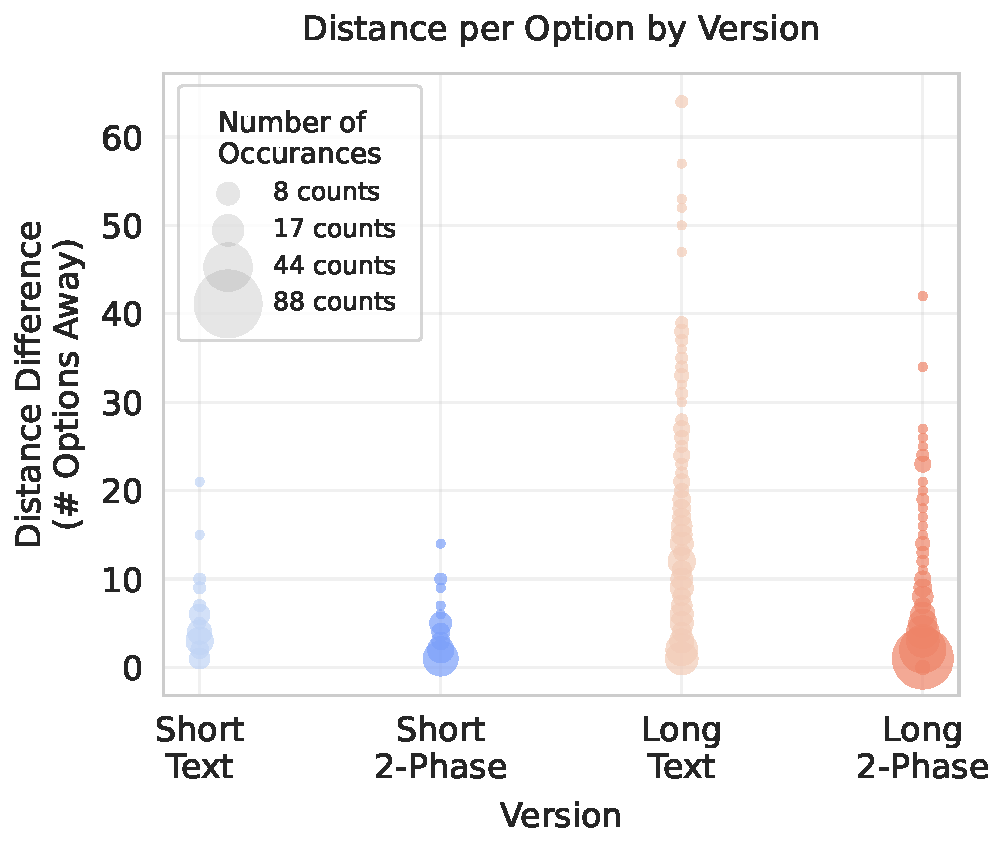
\includegraphics[width=0.5\textwidth]{content/image/distance/distance_diff_by_version.pdf}
    \caption{Edit Distance Per Option: We sum the total number of edit distances for each option, with the figure using the radius to indicate how often a specific edit distance occurred within an experimental condition. Interpretation: Participants in the two-phase interface completed their votes for more options with fewer edit distances, whereas the Long Text interface shows a long tail of options requiring a wider range of edit distances.}
    \label{fig:dist_per_option}
\end{figure}

\textbf{Edit distance per option:} We sum up all the distances a participant moves while adjusting values for a single option. Each of these totals is referred to as the edit distance per option. Figure~\ref{fig:dist_per_option} illustrates differences across the four experimental conditions, with the long text interface showing the largest variance in the distance traveled and the highest mean. We implement a hierarchical Bayesian framework to model edit distance differences across experimental conditions. The observed distance differences are modeled using an exponential distribution, where the scale parameter is linked to survey length (treated as an ordinal variable), interface type (treated as a categorical variable), interaction effects between length and interface, and controlling for individual user variability. The linear predictor includes a global intercept and slope for length, random effects for each interface condition with an LKJ prior that captures the correlations among interface categories, and user-specific random effects to account for individual heterogeneity. Detailed mathematical formulations of the model are provided in Appendix~\ref{sec:apdx:model_distance_option}. 

\begin{figure}[ht]
    \centering
    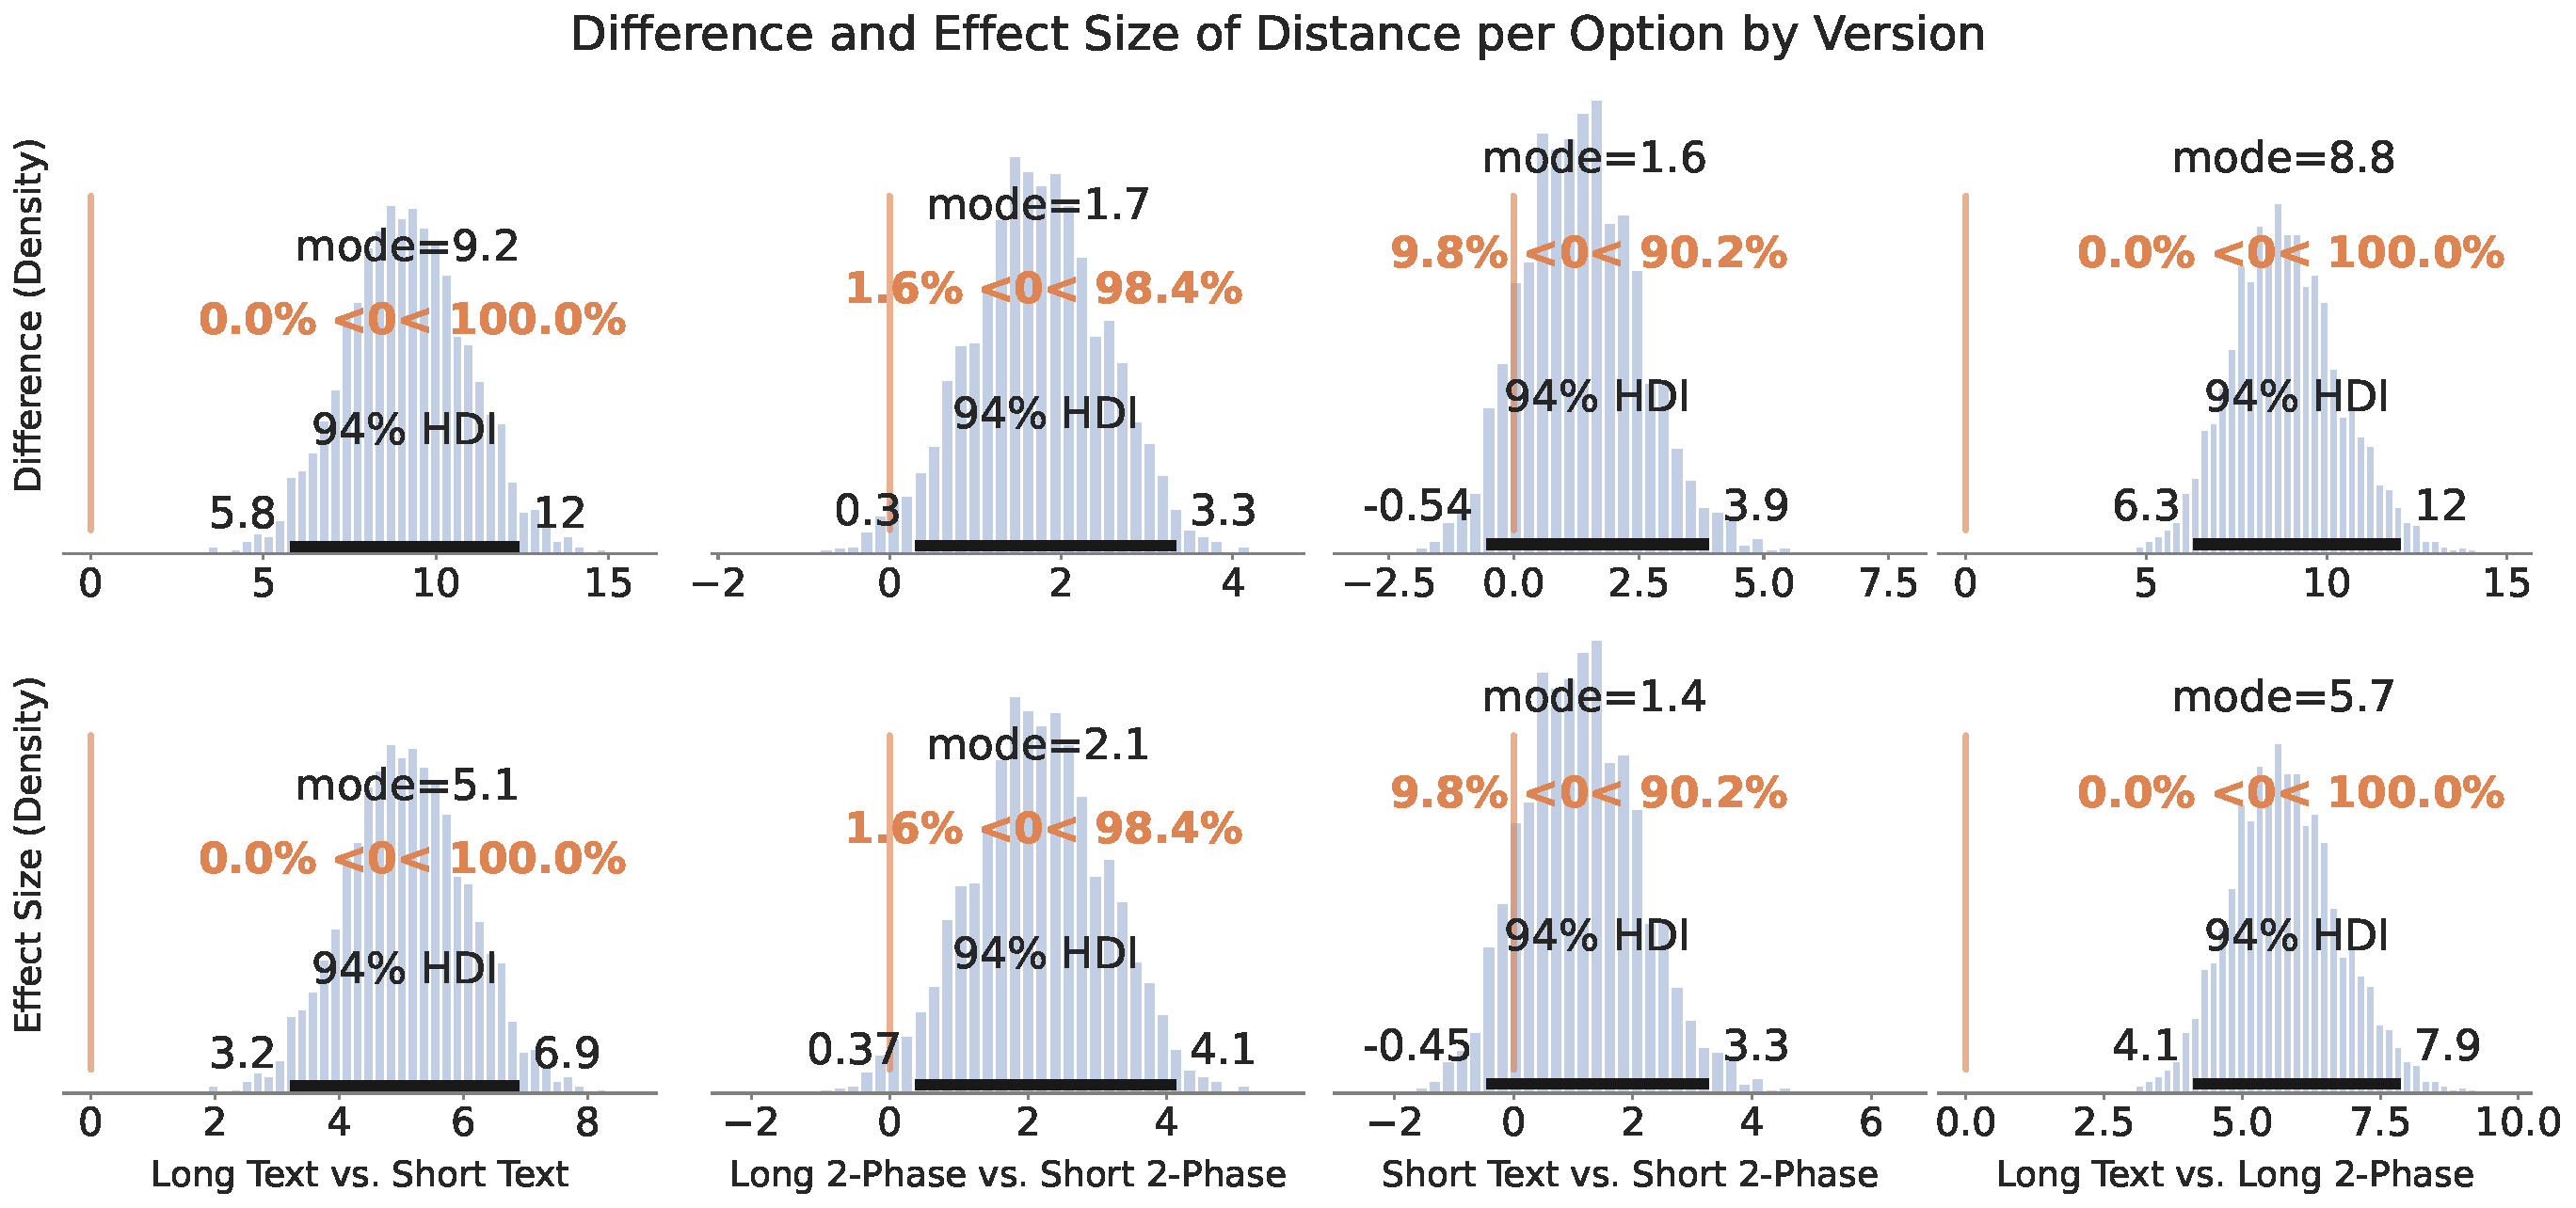
\includegraphics[width=0.9\textwidth]{content/image/distance/distance_diff_per_option_effect_size_by_version.pdf}
    \caption{The figure shows the contrast distributions of the mean edit distance per option between pairwise experimental conditions, with the first row representing absolute differences and the second row depicting effect sizes. The main finding is that participants in the long text estimated more edit distance per option compared to those in the short text and the long two-phase condition. Notably, the long two-phase interface required estimated only slightly more edit distances despite the longer survey length.}
    \label{fig:dist_per_option_bayesian}
\end{figure}


Figure~\ref{fig:dist_per_option_bayesian} illustrates the pairwise posterior distributions for differences in edit distances across experimental conditions. For example, the difference in edit distances between the short and long static interfaces has a mode of 9.1, with a 94\% highest density interval (HDI) of [6, 13]. This indicates that participants in the long text interface move approximately 9.1 steps more than those in the short text interface, with a high degree of confidence. The effect size is large (mode = 5.1, 94\% HDI = [3.3, 7.1]), suggesting a statistically significant difference, which is expected due to the greater number of options in the long text interface.

Similarly, participants using the two-phase interface make approximately 8.9 fewer steps per option (mode = 8.9, 94\% HDI = [6.4, 12]) compared to those in the long text interface, with a large effect size (mode = 5.7, 94\% HDI = [4.2, 7.9]). Comparatively, the increase in edit distances between the short and long two-phase interfaces is substantially smaller (mode = 1.7, 94\% HDI = [-0.01, 3.1]) compared to their static counterparts discussed above. The comparison between the short text and short two-phase interfaces shows weak evidence for a difference, with a mode of 1.3 and a 94\% HDI of [-0.78, 3.8]. While the interval includes zero, the posterior distribution slightly favors (with 89.3\% probability) the two-phase interface requiring fewer steps. Results from this model suggest that the organization phase in the two-phase interface reduces participants' edit distance per option on average, especially for the long QS.

\begin{figure}[h]
    \centering
    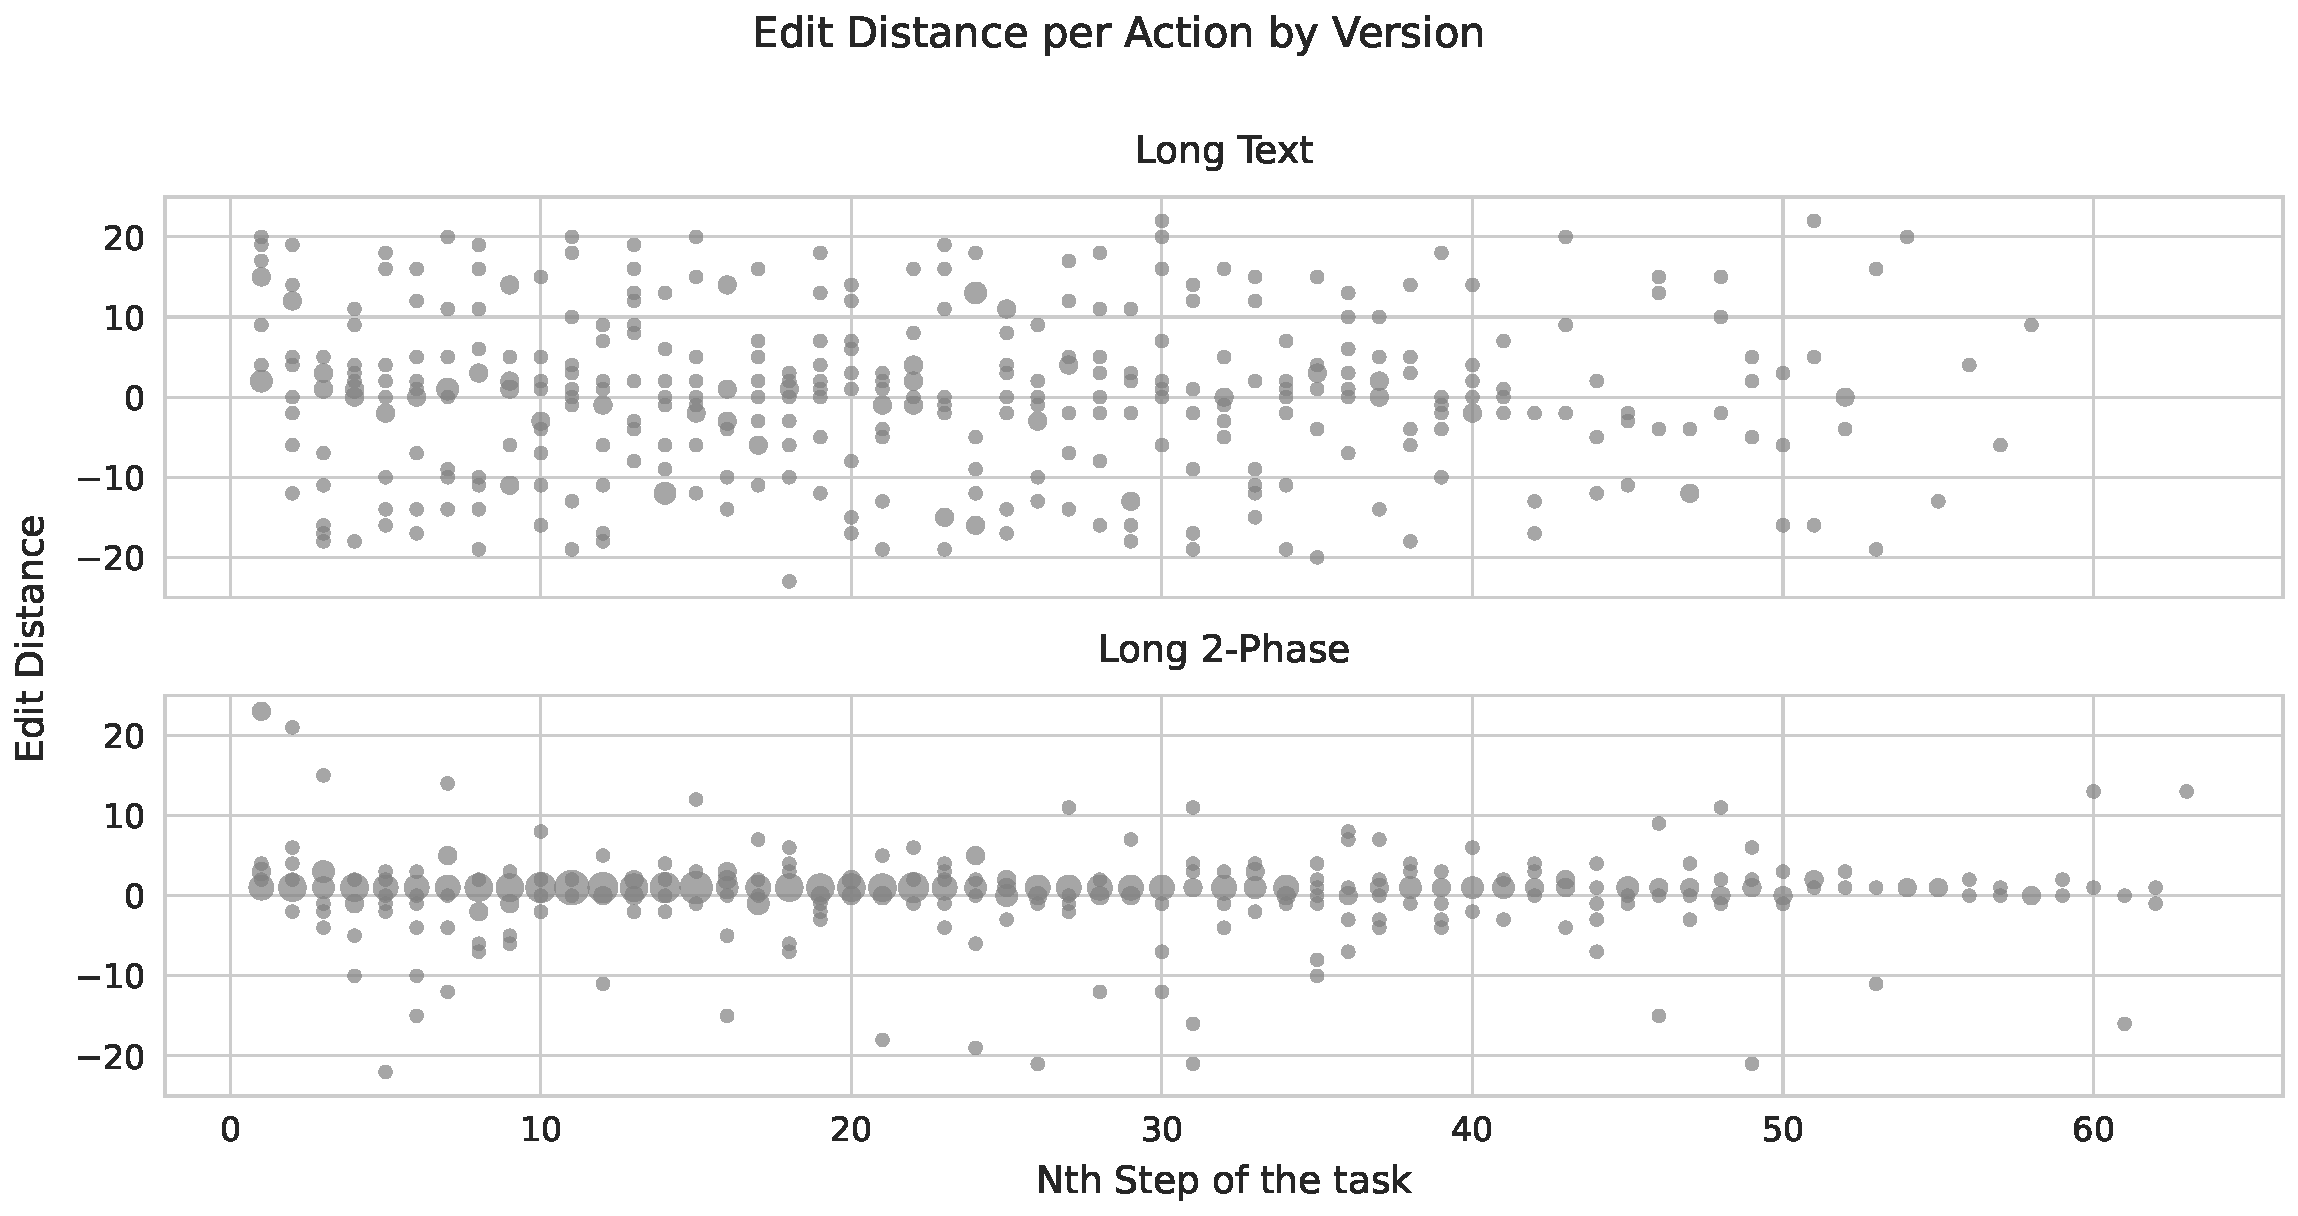
\includegraphics[width=0.8\textwidth]{content/image/distance/edit_distance_per_action_by_version.pdf}
    \caption{Edit Distance Per Action: This plot shows the frequency of specific edit distances at each step across the text interface and two-phase interface. Interpretation: Participants in the long two-phase interface tend to make adjustments closer to their previous actions, resulting in visually less variance in edit distances throughout the entire survey.}
    \label{fig:step-over-distance}
\end{figure}

\textbf{Edit distance per action:} Building on the statistical disparities observed in the previous analysis and the unique patterns exhibited by long text interface participants, we present analyses focusing on edit distance per action and cumulative edit distance throughout the survey between the long text and long two-phase interfaces. Edit distance per action measures how far participants move during each adjustment while completing the survey. Figure~\ref{fig:step-over-distance} illustrates how, at each step, the number of participants moving a given distance (represented by the size of the dots) varies across experimental conditions. Visually, participants move less on average per option within the two-phase interface, with lower variance at smaller scales. This indicates that participants are making local edits, meaning their adjustments tend to occur near their previous edits in terms of edit distance. This also highlights that the organization phase effectively adjusts option positions for easier access, despite participants still having the freedom to move across the interface as all options are presented to them.

In contrast to earlier analyses, we use a hierarchical Bayesian model (detailed in Appendix~\ref{sec:apdx:model_distance_variance}) to jointly estimate the mean and variance of edit distances across experimental conditions. The model assumes that edit distances are continuous and follow a Normal likelihood. This approach accounts for both central tendencies and variability, using separate predictors for the mean and variance. The model includes hierarchical effects for survey length, interface type, interactions between length and interface, and user-level random effects. Non-centered parametrization is used for survey length and interface type to improve convergence, while interaction effects are modeled with an LKJ prior to capture the correlations between factors. User-level random effects reflect individual differences in behavior, incorporating variability into the model.

\begin{figure}[h]
    \centering
    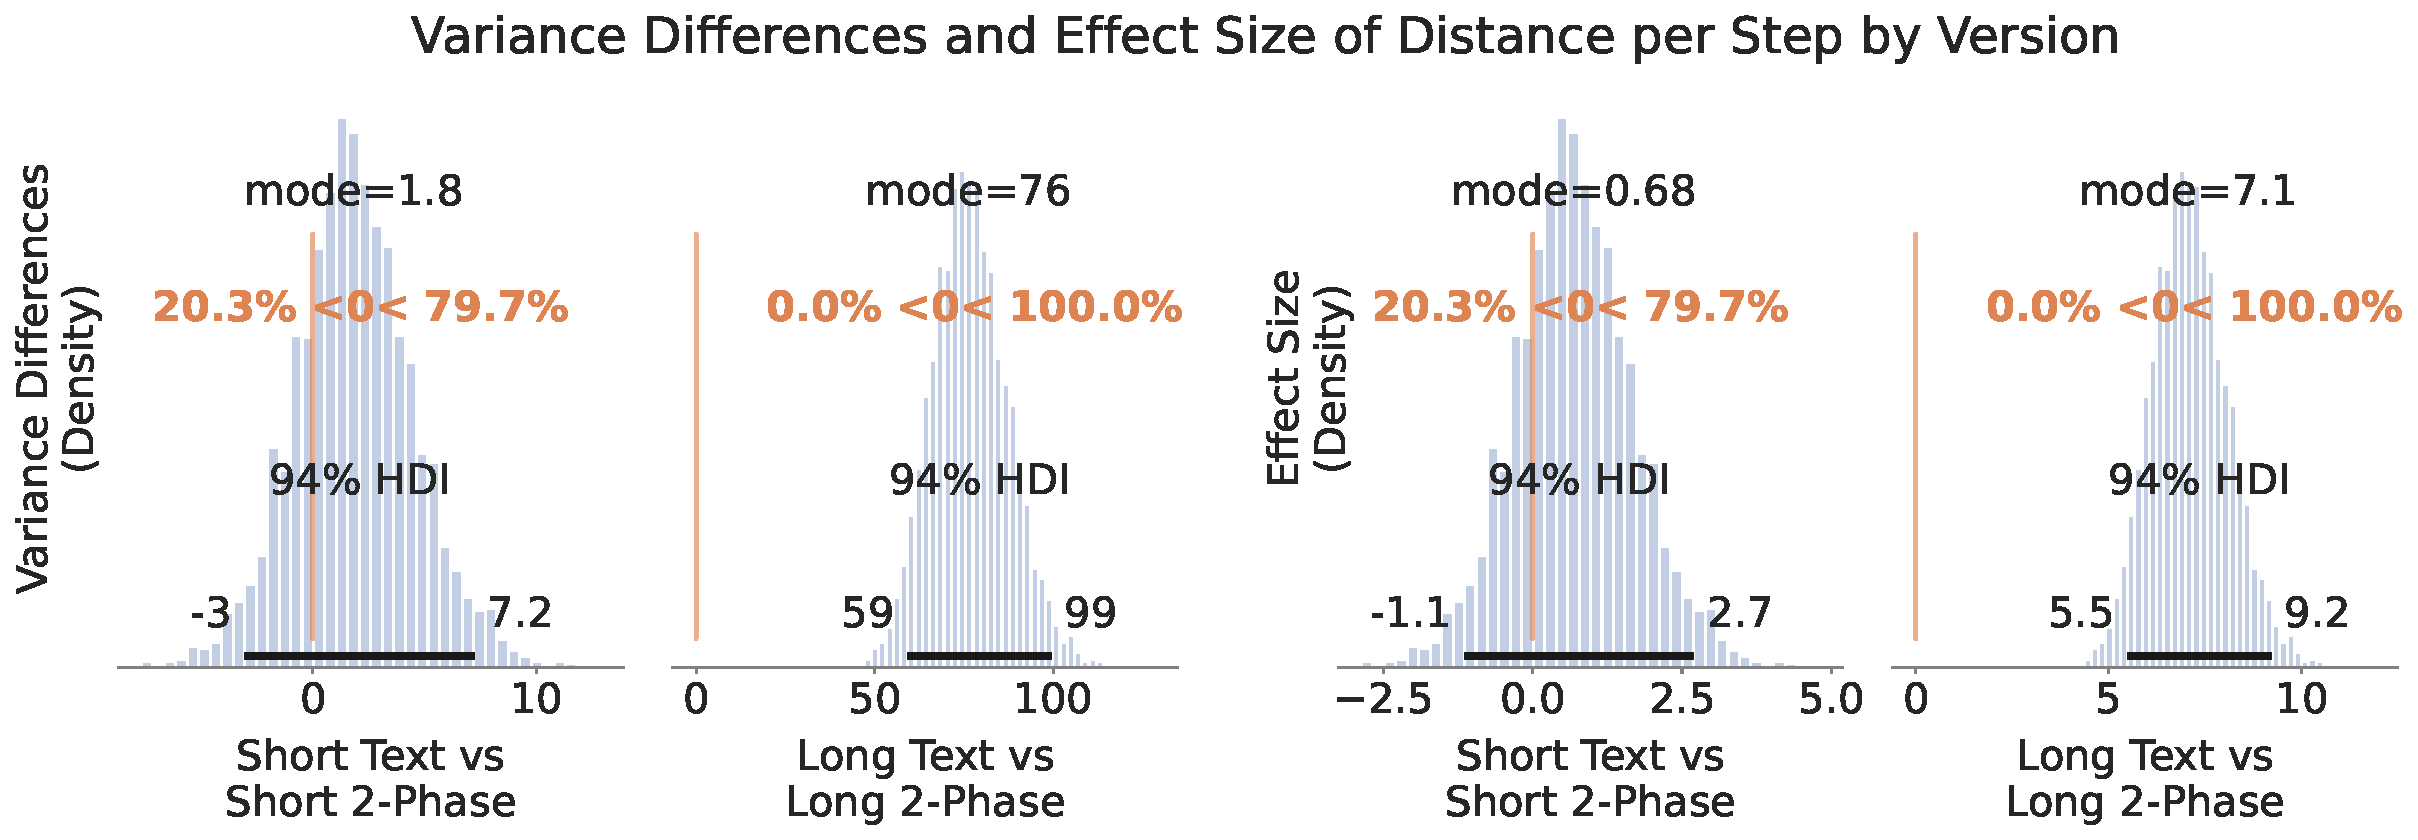
\includegraphics[width=0.8\textwidth]{content/image/distance/distance_diff_per_step_effect_size_by_version.pdf}
    \caption{The figure shows the contrast distributions of the mean edit distance per step between the two-phase interface and text interface for different survey lengths. The left two subplots represent absolute differences, while the right two depict effect sizes. The main finding is that participants in the long text condition exhibited greater variance in edit distance per step compared to those in the long two-phase interface. Similarly, the short text condition showed higher differences, although these were not statistically significant in Bayesian terms.}
    \label{fig:step-over-distance_bayesian}
\end{figure}

Figure~\ref{fig:step-over-distance_bayesian} illustrates the posterior variance distributions, confirming our hypothesis. Participants in the long text interface exhibit greater variance in movement, frequently navigating across the interface, compared to those in the long two-phase interface. This is evidenced by a variance difference mode of 76 (95\% HDI = [59, 99]) and a large effect size (mode = 7.1, 95\% HDI = [5.5, 9.2]).

\begin{figure}[h]
    \centering
    \begin{minipage}[t]{0.48\textwidth}
        \centering
        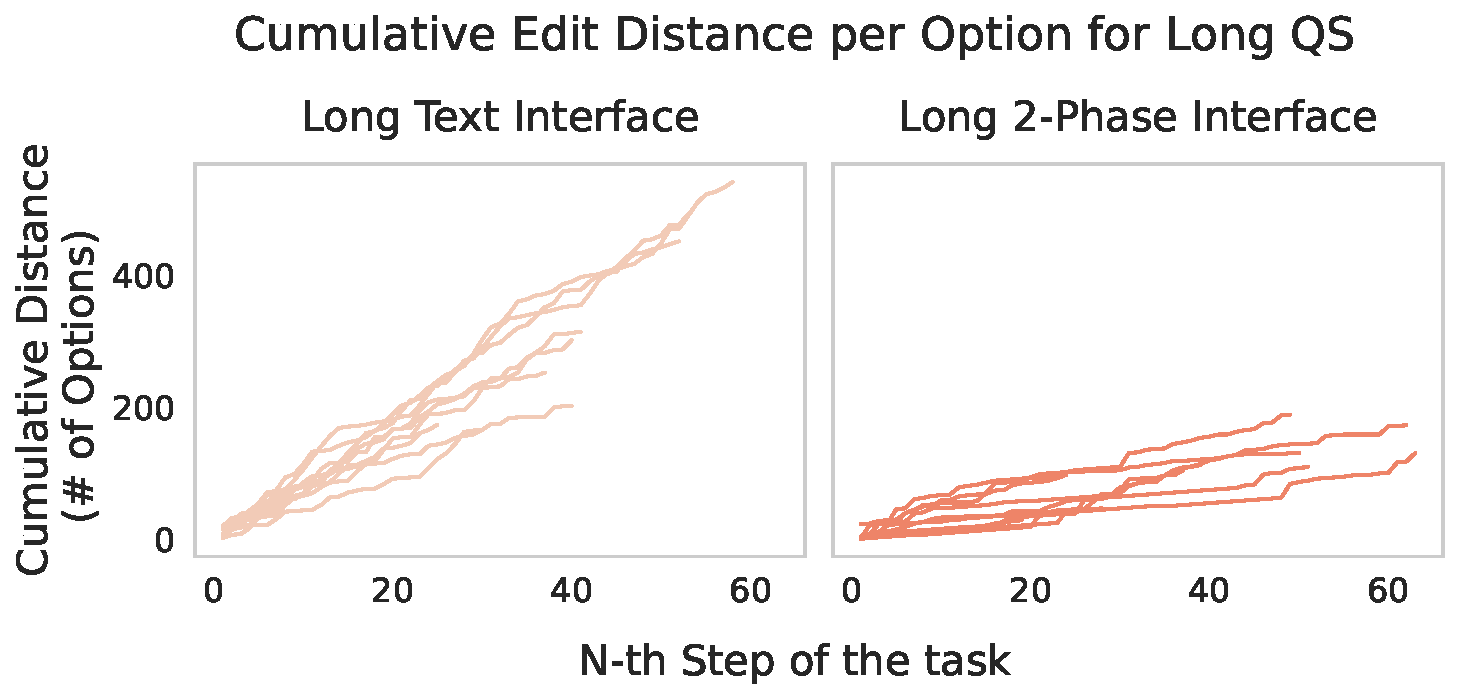
\includegraphics[width=\textwidth]{content/image/distance/cumulative_edit_distance_per_option_long_qs_v3v4.pdf}
        \caption{This plot shows how the cumulative edit distances gained over the course of the survey between long text and long interactive groups. Interpretation: Participants in the long two-phase interface tend to make smaller, more incremental adjustments, resulting in a visually flatter slope compared to the text interface.}
        \label{fig:cumulative-distance}
    \end{minipage}
    \hfill
    \begin{minipage}[t]{0.48\textwidth}
        \centering
        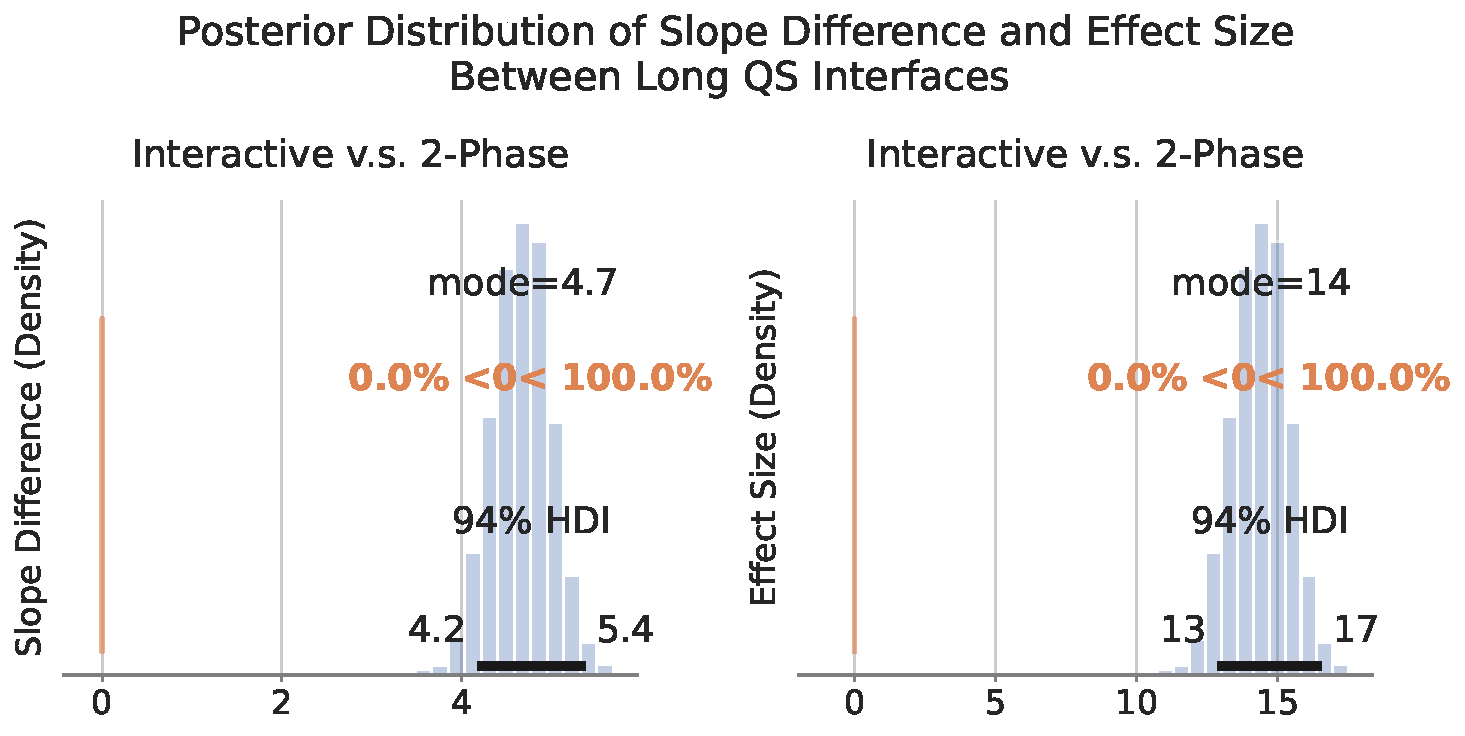
\includegraphics[width=\textwidth]{content/image/distance/slope_diff_and_effect_size.pdf}
        \caption{The figure shows the contrast distributions of slope differences in cumulative edit distance between the two-phase interface and text interface for long QS. The left subplots show absolute differences, while the right depict effect sizes. Main Finding: Participants in the long text interface exhibited a steeper slope, indicating a faster increase in cumulative edit distance compared to the long two-phase interface.}
        \label{fig:slope-diff-effect}
    \end{minipage}
\end{figure}


\textbf{Cumulative edit distance for a participant:} This reduction in per action distance due to the two-phase interface's effect on edit distance adds up, as Figure~\ref{fig:sum-distance} shows the cumulative edit distance over time. Some long text participants traverse double the amount of distance to complete the task compared to the long two-phase participants. We model this growth rate using a hierarchical Bayesian regression model (Detailed in Appendix~\ref{sec:apdx:model_cum_distance}), with cumulative distance as the predictive variable. The experimental variables include interface type as a categorical variable, individual users modeled with random effects, and steps taken as a continuous variable. The model incorporates a shared global intercept, version-specific intercepts and slopes with partial pooling to balance data across conditions, and user-specific random effects to capture variability. A truncated normal likelihood constrains cumulative distances to positive values and varies these distances across steps for each participant while masking incomplete data.

Figure~\ref{fig:slope-diff-effect} shows that the slope for the long text interface is approximately 4.7, meaning each step by the text interface would add 4.7 edit distance (94\% HDI = [4.2, 5.4]), compared to the long two-phase interface, which shows a statistically significant difference with a mode of 1.4 (94\% HDI = [1.3, 1.7]). These results explain that the variance in edit distance per action and the increase in per option edit distance are consistent across participants between the two groups, showing that the organization phase allows participants to focus on adjusting options within proximity without having to navigate the interface to locate and make adjustments during the voting phase.

\textbf{Evidence from qualitative analysis:} Recall the differences in sources of cognitive load between the two experimental conditions: while two-phase interface participants make adjustments with nearby options, they experience cognitive demand from preference construction due to broader considerations involving more options and higher-order values. Similarly, the qualitative results highlight that long text interface participants construct narrower preferences, yet their edit distance indicates that their movements cover more options.

Notably, fewer participants (60\%, N=6) report precise resource allocation in the long two-phase interface compared to 90\% in the long text interface. These results make it evident that two-phase interface participants are more focused on deliberating preferences than simply completing the survey. Furthermore, the ability to make localized adjustments while considering broader decisions suggests that participants construct preliminary preferences during the grouping phase, allowing them to focus on deciding their votes.

These results provide evidence that the initial pass through the survey items, combined with the organizational phase, helps participants construct preliminary preferences, thereby reducing the need for large traversals between options. This could exemplify that participants in the long text interface are more concerned about operating to 'complete' the task (i.e., looking for an option to adjust votes) rather than continuing to stay engaged with the survey options and the preference construction task, particularly in the long survey.



% Physical demand refers to the physical effort required to complete a task, such as physical exertion or movement. The two-phase interface experienced higher physical demand from increased mouse usage.

% \begin{displayquote}  
% Because with this many (options), especially when I'm thinking \ldots\ Ok, where was (the option) \ldots\ Where was (the option) you know? Oh, that's right. Maybe I could give another upvote to the, you know, whatever~\bracketellipsis \hfill\quoteby{S028 (LT)}  
% \end{displayquote}  